%
% HICSS-60 initial submission -- double-blind
%
% Title: Deterministic-Dimension Reduction for Reliable LLM Agents:
%        A Design-Science Study of Spatial Construction and Edge Deployment
%
% Author block omitted per HICSS double-blind requirements.
% Repository references anonymized per HICSS double-blind requirements.
%

\documentclass[10pt]{article}
\usepackage[letterpaper]{geometry}
\usepackage{hicss}
\usepackage{times}
\usepackage[none]{hyphenat}
\usepackage{url}
\usepackage{latexsym}
\usepackage{indentfirst}
\usepackage{graphicx}
\graphicspath{{../dist/abstract/figures/}{images/}}
\usepackage{amsmath}
\usepackage{amssymb}
\usepackage{booktabs}
\usepackage{enumitem}
\usepackage{orcidlink}
\usepackage[
    style=apa,
    backend=biber,
    apamaxprtauth=11,
]{biblatex}
\addbibresource{references.bib}


\setlength\titlebox{6cm}

\title{Deterministic-Dimension Reduction for Reliable LLM Agents:\\
A Design-Science Study of Spatial Construction and Edge Deployment}

\date{}

\begin{document}

\maketitle

\begin{abstract}
Reliable language model agents in physically constrained domains often
assign output dimensions to the model that are deterministic functions of
task state. We introduce deterministic-dimension reduction, a design
principle in which such dimensions are computed outside the model by a
symbolic executor, reducing the model to language understanding and plan
generation while eliminating entire error classes. We instantiate the
principle in a 2.5-D spatial construction agent: the model plans in the
horizontal plane while a deterministic executor computes vertical placement
from column occupancy. Across the Build What I Mean benchmark, a component
ablation, cross-model comparison, IGLU transfer, and edge deployment on
embedded AI hardware, we find that architectural decomposition improves
reliability more than model scaling alone. A small, low-cost model with the
decomposition architecture matches or exceeds a frontier model generating
coordinates directly. We extract five design implications for reliable,
cost-aware, and deployable agentic systems.
\end{abstract}

\subsubsection*{Keywords:}
large language models, reliable AI agents, neuro-symbolic systems,
design science, spatial reasoning

% ============================================================
\section{Introduction}
% ============================================================

Language model agents operating in physically constrained domains face a
structural reliability problem. These domains impose constraints that make
some output dimensions computable rather than learnable, yet standard agent
architectures ask the model to generate all output dimensions equally. The
model then routinely produces errors in exactly the dimensions it did not
need to generate at all.

Consider a block construction agent that must place colored blocks in a
gravity-bound grid. The vertical coordinate of any new block is a
deterministic function of column occupancy: a block placed at horizontal
position $(x, z)$ always lands at the first unoccupied height in that
column. An LLM asked to generate full three-dimensional coordinates must
nonetheless compute this value, and off-by-one height errors, duplicate
placements, and miscounted stack heights are the predictable result
\parencite{yamada2024, bang2023}. The same structural issue arises in
other constrained domains. In terrain-following path planning, altitude is
a function of horizontal position and terrain data. In robotic assembly
with geometric constraints, some degrees of freedom are determined by
constraint equations once the free dimensions are fixed. In automated code
generation, syntax rules and type constraints determine many tokens that
language models nonetheless produce incorrectly.

We propose deterministic-dimension reduction, a design principle for
agentic systems: identify output dimensions that are deterministic functions
of task state and current output, remove them from the language model's
generation space, and compute them using a symbolic executor. This reduces
the model to language understanding, ambiguity resolution, and structured
planning, while eliminating entire classes of output error.

We instantiate the principle in a 2.5-D spatial construction agent and
evaluate it on the Build What I Mean (BWIM) benchmark \parencite{bwim},
a publicly scored competition requiring block structure construction from
natural-language instructions. The agent plans exclusively in the
horizontal plane while a deterministic executor computes vertical
placement via column occupancy. This 2.5-D decomposition, named by
analogy with \textcite{marr2010}'s 2.5-D sketch and with 2.5-D machining
\parencite{held1991}, eliminates $y$-coordinate errors entirely.

An earlier conference version of this work presents the 2.5-D spatial
construction method and a compact benchmark evaluation. The present paper
extends that contribution by developing the deterministic-dimension
reduction design principle, adding edge-deployment and latency evidence,
IGLU cross-benchmark transfer, and design implications for reliable
agentic systems. Citation omitted for blind review.

This paper addresses three design questions. First, does removing
deterministic output dimensions from an LLM agent improve reliability
in a constrained construction domain, and which pipeline components
contribute most? Second, does a decomposed architecture reduce dependence
on large frontier models, and does it remain viable on cost-constrained
and edge hardware? Third, under what conditions does the principle apply,
and does the pattern recur in agent domains beyond spatial construction?
The first two questions are addressed through controlled experiments on the
BWIM benchmark. The third is addressed through an IGLU cross-benchmark
transfer experiment and through design observations in two additional
agentic systems described in Section~\ref{sec:crossdomain}, with the
distinction between experimental and observational evidence noted
throughout.

The contributions of this paper are: (1) the deterministic-dimension
reduction design principle, including a formal analysis of multiplicative
error accumulation on deterministic output dimensions showing that a
symbolic executor strictly dominates the language model for any positive
error rate, and a taxonomy of three categories of deterministic operations
in agentic systems, (2) a 2.5-D construction agent as a controlled
instantiation of the principle, (3) a decision-theoretic framework for
underspecification handling under asymmetric scoring, (4) a multi-context
evaluation spanning benchmark accuracy, component ablation, model-cost
tradeoff, edge deployment, and cross-dataset transfer, and (5) design
implications for reliable, cost-aware, and deployable agentic systems,
supported by design observations from two additional agentic systems
suggesting the principle recurs across agent domains.

% ============================================================
\section{Background}
% ============================================================

\subsection{LLM Spatial Reasoning Limitations}
Large language models exhibit systematic weaknesses in spatial and
directional reasoning. \textcite{yamada2024} benchmark LLMs on spatial
tasks and find that coordinate tracking and relative positioning are
persistent error sources. \textcite{bang2023} document directional and
chain-reference failures in GPT-family models. \textcite{lecun2022}
observes that LLMs lack internal world models for enforcing physical
constraints. These weaknesses are especially pronounced in 3D construction
tasks, where the model must track block occupancy across three axes and
chain height calculations across stacking operations.

\subsection{Neuro-Symbolic and Decomposed Approaches}
The neuro-symbolic tradition addresses these limitations by separating
neural and symbolic computation. \textcite{yi2018} decompose visual
question answering into a neural perception module and a symbolic
execution engine. \textcite{wang2023} show that separating planning from
execution improves zero-shot reasoning. \textcite{khot2023} split complex
tasks into sub-problems handled by specialized modules. Our approach
extends this work by exploiting a dimensional constraint: the planning
module operates in 2D while execution operates in 3D, a separation not
explored in prior decomposed-prompting work.

\subsection{Tool Use and Robotic Grounding}
\textcite{schick2023} demonstrate that language models can learn to invoke
external tools. \textcite{saycan2022} ground language model plans in
robotic affordances, restricting the LLM to skills the robot can
physically perform. \textcite{cap2022} have the LLM generate code that
calls spatial APIs directly, offloading coordinate arithmetic to
deterministic libraries. \textcite{innermonologue2022} close the loop
with environment feedback for replanning. Our approach shares the
principle of restricting LLM outputs to what deterministic modules can
process reliably, but identifies a specific dimensional constraint, the
gravity axis, rather than grounding arbitrary skills or generating full
executable code.

\subsection{Offloading Deterministic Computation from LLMs}
A parallel line of work argues that language models should not generate
output values that are computable by a deterministic procedure, because
delegating computable dimensions to the language model introduces
avoidable error. \textcite{pal2023} show that separating language-level
reasoning from arithmetic computation and executing the arithmetic in a
Python interpreter eliminates computational errors entirely, with
improvements of over 10 percentage points on average across numerical
benchmarks. \textcite{pot2023} make the same argument under the label
``disentangling computation from reasoning,'' demonstrating that
systematic errors in LLM-generated arithmetic are avoidable by design
rather than reducible only by scale. \textcite{faithfulcot2023} extend
the principle to symbolic reasoning chains: the language model generates
a structured plan and a deterministic solver executes it, providing a
guarantee of faithful execution that language model sampling cannot
provide.

At a broader architectural level, \textcite{mrkl2022} propose routing
LLM queries to discrete expert modules for reasoning steps that have
known-correct computational procedures. \textcite{kambhampati2024} offer
a near-formal argument that autoregressive generation cannot achieve
correctness guarantees on planning tasks and that symbolic verifiers
or executors are required at every constrained step.
\textcite{dziri2023} show empirically and theoretically that transformer
performance degrades with the compositional depth of a task, consistent
with errors accumulating across chained generative steps.

These works collectively support the design intuition underlying
deterministic-dimension reduction: removing a computable output dimension
from the LLM's generation space eliminates its associated error class
rather than reducing it. The present paper extends this line by providing
a formal characterization of when and why this dominance holds,
introducing the free-dimension and deterministic-dimension decomposition
as an explicit design vocabulary, and applying it to a constrained
construction domain with controlled ablation evidence.

\subsection{Design Science}
Design science research produces artifact knowledge: design principles,
methods, and constructs that expand what is achievable in practice
\parencite{hevner2004}. The design-science framing is appropriate here
because the primary contribution is not a benchmark result but a design
principle applicable beyond any single domain or benchmark.

% ============================================================
\section{Deterministic-Dimension Reduction}
% ============================================================

\subsection{Design Principle}

Let the agent's output for a given task instance be a tuple
$o = (v_{\mathrm{free}}, v_{\mathrm{det}})$, where
$v_{\mathrm{free}} \in D_{\mathrm{free}}$ denotes the \emph{free dimensions}
and $v_{\mathrm{det}} \in D_{\mathrm{det}}$ denotes the \emph{deterministic
dimensions}. The free dimensions are those that require language
understanding, disambiguation, or reasoning about intent: they cannot be
computed from task state alone and constitute the genuinely generative part
of the task. The deterministic dimensions are those whose correct value is
fully determined by task state $s$ and the free dimensions already chosen:
\[
  v_{\mathrm{det}} = f(s,\, v_{\mathrm{free}})
\]
for some computable function $f$. In block construction, $v_{\mathrm{free}}$
is the horizontal position $(x, z)$ and block color $c$, which require
understanding the natural-language instruction. $v_{\mathrm{det}}$ is the
vertical coordinate $y$, which follows from column occupancy regardless of
instruction content.

In a standard agent architecture the language model generates both
$v_{\mathrm{free}}$ and $v_{\mathrm{det}}$. This is unnecessary for the
deterministic dimensions and costly in practice. A language model sampling
$v_{\mathrm{det}}$ from its output distribution produces the correct value
with probability $1 - \varepsilon$ for some model-specific error rate
$\varepsilon > 0$. A symbolic executor computing $f(s, v_{\mathrm{free}})$
produces the correct value with probability 1, provided $v_{\mathrm{free}}$
is correct and $f$ is implemented correctly. There is no tradeoff: for any
$\varepsilon > 0$, the symbolic executor strictly dominates the language
model on the deterministic dimensions. When errors compound across multiple
deterministic dimensions per output, the advantage grows multiplicatively.

Deterministic-dimension reduction restricts the model's output schema to
$D_{\mathrm{free}}$ and delegates $D_{\mathrm{det}}$ to a symbolic
executor. This has three further consequences beyond error elimination.
The model's output space shrinks, reducing the burden on context and
sampling. Smaller models that perform adequately on $D_{\mathrm{free}}$
can match larger models that must additionally produce $D_{\mathrm{det}}$.
The symbolic executor is independently testable and verifiable, separating
evaluation of the language understanding component from evaluation of the
execution component.

\subsection{Applicability Conditions}

The principle applies when: (a) one or more output dimensions are
deterministic functions of task state and the remaining output, (b) the
function $f$ is computable in closed form or by a finite algorithm, and
(c) the LLM makes systematic errors in $D_{\mathrm{det}}$ despite correct
$D_{\mathrm{free}}$ outputs.

Condition (c) is the practical trigger. In gravity-bound construction,
$y$-coordinates satisfy (a) and (b) trivially, and LLMs routinely produce
$y$-errors even when horizontal placement is correct, satisfying (c). In
UAV altitude control over terrain, altitude satisfies (a) and (b) given
terrain data, and altitude errors are a known failure mode in LLM path
descriptions. In code generation, bracket matching and type consistency
satisfy (a) and (b), and token-level syntax errors in LLM output satisfy
(c). The same pattern applies to any system with physical or logical
constraints that fix some output dimensions once the free dimensions are
determined.

\subsection{A Taxonomy of Deterministic Operations}

Agent domains exhibit at least three categories of deterministic
operations, distinguished by the source of the constraint.

\subsubsection{Geometric and Physical Constraints}
The constraint follows from a law of the domain. Gravity determines
vertical placement in block construction. Terrain data determines
altitude in path planning. Kinematic equations limit reachable positions
in robotic assembly. These constraints apply globally to every task
instance. The LLM adds no value in computing them and produces systematic
errors when asked to do so.

\subsubsection{Procedural Knowledge Constraints}
The constraint is a codified rule that follows deterministically from
observable input properties. In tabular machine learning, the correct
handling of a null-valued boolean column is determined by the column's
dtype and null statistics, not by language model judgment. Published best
practices for machine learning engineering codify many such rules
\parencite{zinkevich2017}: given data properties, preprocessing steps are
a function of those properties, not a generation task. In code generation,
bracket matching and type-consistency rules are similarly determined by
language grammar rather than by content.

\subsubsection{Workflow State Management Constraints}
The constraint is a protocol with a known-correct execution sequence.
Git fetch must precede checkout. Build must precede test. Test must precede
merge. These sequences are fully determined before the agent runs, require
no language model reasoning, and produce omission and sequencing errors
when delegated to the LLM.

Section~\ref{sec:crossdomain} presents design observations from two
agentic systems where this taxonomy was applied in separate project
contexts.

% ============================================================
\section{Artifact: 2.5-D Construction Agent}
% ============================================================

\subsection{Task and Benchmark}

The BWIM benchmark defines a block construction task on a discrete grid
$\mathcal{G} = \{0,\ldots,8\} \times \{0,\ldots,4\} \times \{0,\ldots,8\}$
where each cell is either empty or occupied by a colored block. In each
round, the builder agent receives a natural-language instruction and a
starting grid state, and must produce a target grid state. The agent may
ask one clarification question before building. The scoring function
awards $+10$ for a correct build, $-10$ for an incorrect build, and $-5$
per question, creating an expected value of $+5$ for a correct build with
one question and $-5$ for an incorrect build with one question.

\begin{figure}[t]
  \centering
  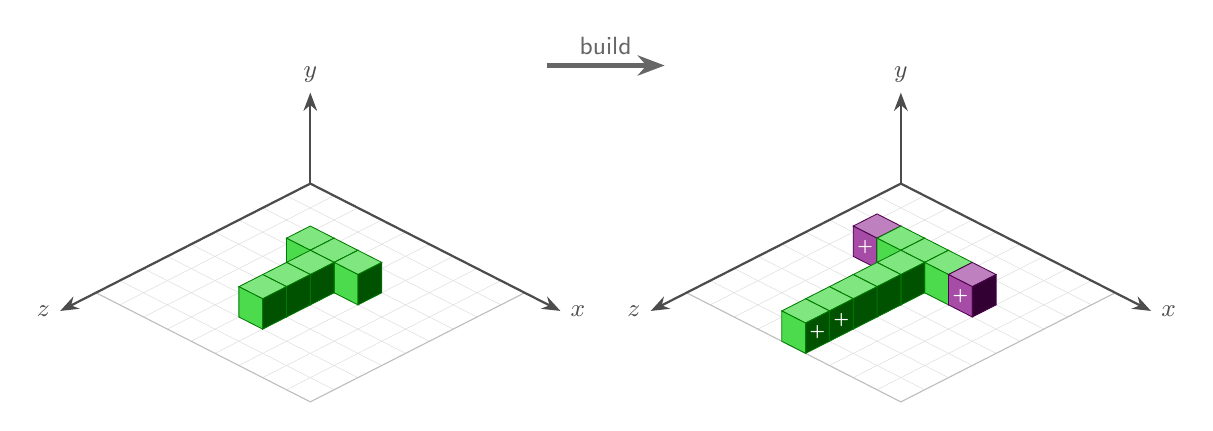
\includegraphics[width=\columnwidth]{tshape_example}
  \caption{A representative BWIM benchmark round involving T-shape
  geometry.}
  \label{fig:tshape}
\end{figure}

\subsection{Instantiating the Principle}

Figure~\ref{fig:tshape} shows a representative benchmark round. The
agent receives a natural-language instruction referencing an existing
green T-shape and must identify its stem and arms, extend the stem by
two blocks, and place a purple block at each arm endpoint. The 2D plan
specifies only horizontal positions and colors. Vertical placement is
computed by the deterministic executor from column occupancy.

The BWIM grid is a 2.5-D domain in the sense of \textcite{marr2010}: the
vertical axis is not a free variable but a deterministic function of
horizontal position and column occupancy. A block at $(x, y, z)$ can only
exist if $y = 0$ or a block exists at $(x, y-1, z)$. The vertical
coordinate of any new block is therefore:
\begin{equation}
  y^*(x, z, G) = \min\{y \in \{0,\ldots,4\} \mid (x, y, z) \notin
  \mathrm{dom}(G)\}
  \label{eq:ystar}
\end{equation}
where $\mathrm{dom}(G)$ is the set of occupied cells. Applying
deterministic-dimension reduction assigns $y^*$ to the symbolic executor
and restricts the LLM to horizontal positions $(x, z)$ and block colors
$c$.

The LLM produces a plan $P = \langle a_1, \ldots, a_k \rangle$ where each
action $a_i$ specifies an action type (stack, place-relative, extend-row),
a horizontal position $(x_i, z_i)$, a color $c_i$, and an optional count
$n_i$. No $y$-coordinate appears anywhere in the plan format.

\begin{figure}[t]
  \centering
  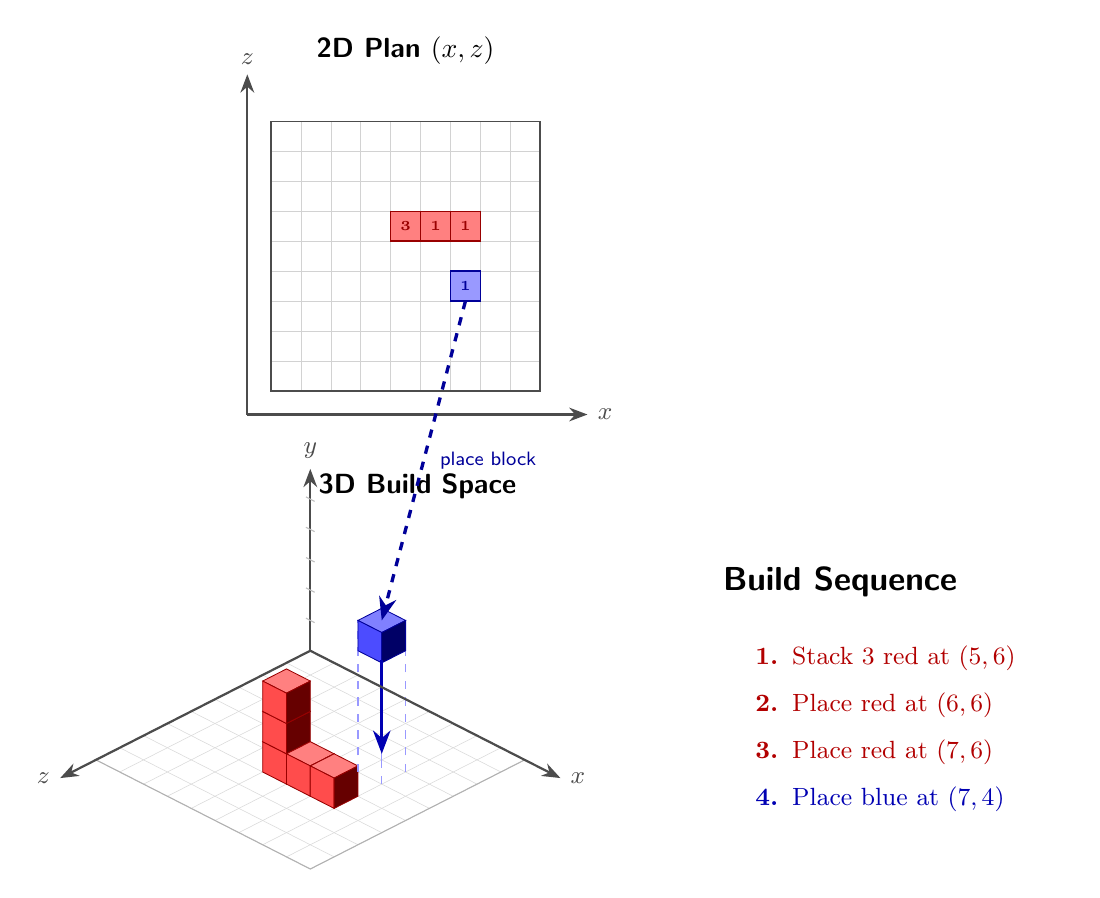
\includegraphics[width=\columnwidth]{25d_decomposition}
  \caption{2.5-D decomposition. The LLM planner generates 2D plans with
  $(x, z)$ coordinates and action types. The deterministic executor
  computes vertical placement via column occupancy
  (Equation~\ref{eq:ystar}).}
  \label{fig:decomp}
\end{figure}

\subsection{Pipeline}

The agent processes each instruction through six stages: parse, analyze,
plan (LLM call), verify, execute (deterministic), and format. The
structure analyzer pre-computes geometric primitives in the starting grid
(rows, stacks, L-shapes, T-shapes) and injects named shape descriptions
into the planner prompt, so the LLM reasons over geometry rather than raw
coordinate lists. Nine worked examples in the system prompt
\parencite{wei2022} cover chains, L-shapes, T-shapes, and edge placements.
No example includes $y$-coordinates. The spatial executor processes each
action, computes $y$ via Equation~\ref{eq:ystar}, and chains positional
context across steps. No LLM call is involved at execution time.

A rule-based plan verifier runs four deterministic correction passes before
execution: direction consistency, endpoint cap correction, T-shape axis
correction, and stacking plausibility. These are analogous to peephole
optimization \parencite{mckeeman1965}: known-bad output patterns in the
LLM plan are rewritten deterministically without a second LLM call.

\subsection{Underspecification Handling}

Many BWIM instructions omit color or block count. The scoring function
creates an asymmetric decision problem. Let $p$ denote the probability of
a correct unaided guess. The expected values are:
\begin{align}
  \mathrm{EV}_{\mathrm{guess}}(p) &= 20p - 10 \label{eq:ev_guess} \\
  \mathrm{EV}_{\mathrm{ask}} &\approx 20 - 15 = 5 \label{eq:ev_ask}
\end{align}
assuming a near-perfect architect. Setting equal and solving yields
indifference threshold $p^* = 3/4$. The agent asks when $p < 0.75$.
Color inference achieves approximately 80\% on inferable cases (above
$p^*$); count inference achieves approximately 65\% (below $p^*$), so the
agent asks whenever a count is underspecified and no question has been
used in the current round. Questions are color-specific to allow the
upstream architect to identify the correct stack.

\subsection{Adaptive Prompt Enrichment}

Certain spatial concepts, including chain references, L-shape extensions,
and T-shape junctions, produce systematic LLM errors. The agent scans
each instruction against 15 pattern-matching rules. When a rule fires, a
targeted correction with a worked example is injected into the prompt
before the LLM call. The rules are independently testable and compose
additively. This methodology is applicable to any domain where LLMs make
systematic, input-predictable errors: identify recurring failure modes,
classify by input trigger, write targeted corrections with examples,
inject dynamically, and validate against regressions.

% ============================================================
\section{Evaluation Design}
% ============================================================

The three design questions are addressed through four controlled
conditions and, for cross-domain generality, through design observations
in Section~\ref{sec:crossdomain}.

\subsection{Reliability and Component Contribution}
BWIM 160-round benchmark, GPT-4o-mini (2024-07-18), $n = 12$ independent
runs. Component ablation ($n = 7$ per condition) removes one pipeline
component at a time from the full system.

\subsection{Model-Scale and Cost}
Head-to-head comparison of GPT-4o-mini and GPT-4o (2024-08-06), $n = 12$
and $n = 6$ respectively, on the identical frozen pipeline. Assumption:
all prompt engineering and enrichment rules were developed against
GPT-4o-mini due to cost constraints. GPT-4o runs use the same pipeline
with no model-specific tuning.

\subsection{Cross-Benchmark Transfer and Edge Deployment}
For transfer, 500 gravity-compatible tasks from the IGLU collaborative
building dataset \parencite{iglu2022} compare a bare coordinate-output
prompt against the 2.5-D decomposed prompt at temperature 0, with no
enrichment rules, plan verifier, or underspecification handling. This
isolates the decomposition contribution on an independent benchmark
($11 \times 9 \times 11$ grid, different instructions). For edge
deployment, Nemotron-3-Super-120B-A12B-NVFP4 \parencite{nemotron2024}
runs locally on an NVIDIA Jetson Thor AGX Developer Kit
\parencite{jetsonthor} via vLLM \parencite{vllm2023} (Blackwell GPU,
Arm Neoverse V3AE CPU) under two conditions: full reasoning with 9
examples, and low-effort reasoning with 13 examples designed to exceed
the model's 8,320-token prefix cache page size.

\subsection{Failure Attribution}
Error attribution across all 1,920 GPT-4o-mini rounds, classifying
failures as builder-origin or architect-origin.

All primary runs use a single frozen code commit. Statistical significance
uses Welch two-sample $t$-tests. Run-to-run variance reflects LLM
sampling non-determinism rather than development changes.

% ============================================================
\section{Findings}
\label{sec:findings}
% ============================================================

\subsection{Reliability and Component Contributions}

Table~\ref{tab:ablation} shows the ablation study. Removing 2.5-D
decomposition produces the largest accuracy drop (50.7 percentage points,
$p < 0.0001$), reducing accuracy to 43.8\%.

This result requires an important clarification. The ablation condition
retains all surrounding control logic from the final architecture,
including enrichment rules and prompt examples designed for 2D output
format. Disabling the deterministic executor while forcing the LLM to emit
full 3D coordinates places an architecture designed for 2D planning into a
format mismatch. The 43.8\% result is therefore lower than an earlier
development baseline that used direct 3D output with a hand-crafted system
prompt (81.9\%, single $n=1$ run without the surrounding pipeline). We
interpret the ablation as measuring the contribution of 2.5-D decomposition
within the final architecture, not as a comparison against all possible
direct-3D configurations.

Underspecification questions contribute the second largest effect
($-17.9$ pp), consistent with the $p^* = 0.75$ threshold. Adaptive prompt
enrichment accounts for $-11.3$ pp and the skip-forward rule for $-3.9$
pp. The plan verifier shows no statistically significant effect ($-0.6$
pp, $p = 0.36$), suggesting enrichment rules prevent most errors the
verifier would otherwise target.

\begin{table}[t]
\centering
\small
\caption{Ablation study ($n = 7$ per condition, GPT-4o-mini). $\Delta$
is relative to the full system.}
\begin{tabular}{@{}lcccc@{}}
\toprule
\textbf{Configuration} & \textbf{Mean} & $\sigma$ & $\Delta$ & $p$ \\
\midrule
Full system ($n=12$)  & 94.6\% & 0.72\% & -- & -- \\
$-$ 2.5-D decomp.     & 43.8\% & 1.42\% & $-$50.7 pp & $<$0.0001 \\
$-$ Underspec.\ qs    & 76.7\% & 0.70\% & $-$17.9 pp & $<$0.0001 \\
$-$ Enrichment        & 83.3\% & 1.29\% & $-$11.3 pp & $<$0.0001 \\
$-$ Skip-forward      & 90.7\% & 1.22\% & $-$3.9 pp  & $<$0.0001 \\
$-$ Plan verifier     & 94.0\% & 1.44\% & $-$0.6 pp  & 0.36 \\
\bottomrule
\end{tabular}
\label{tab:ablation}
\end{table}

\subsection{Model-Scale Dependence and Cost}

Table~\ref{tab:comparison} shows the model comparison. GPT-4o-mini
outperforms GPT-4o by 4.3 percentage points ($p < 0.0001$, Cohen's
$d = 6.8$), a result opposite to what model scaling alone would predict.
This finding should be interpreted with the caveat that prompt engineering
was developed against GPT-4o-mini. Had development been conducted against
GPT-4o from the start, GPT-4o results could plausibly be higher. However,
GPT-4o with the untuned pipeline reaches 90.3\%, well above the best
competing system's 76.3\% using GPT-4o without a decomposition pipeline
\parencite{hisandan}, indicating that the pipeline provides value
independent of model-specific tuning.

GPT-4o incurs approximately 16.7$\times$ higher per-token cost. Each
160-round GPT-4o-mini run costs approximately \$0.07 versus \$1.10 for
GPT-4o, a 16$\times$ cost difference for 4.3 percentage points lower
accuracy on this pipeline.

\begin{table}[t]
\centering
\small
\caption{Model comparison on the frozen pipeline.}
\begin{tabular}{@{}lcccc@{}}
\toprule
\textbf{Model} & $n$ & \textbf{Acc.} & \textbf{Score} & \textbf{F1} \\
\midrule
GPT-4o-mini       & 12 & 94.6\% & $+$947 & .987 \\
GPT-4o            &  6 & 90.3\% & $+$810 & .975 \\
Nemotron-3$^\dag$ &  6 & 96.0\% & $+$993 & .987 \\
\bottomrule
\multicolumn{5}{@{}l@{}}{\footnotesize $^\dag$Local Jetson Thor AGX,
Blackwell GPU, full reasoning.}
\end{tabular}
\label{tab:comparison}
\end{table}

\subsection{Transfer to Independent Benchmark}

On 500 IGLU tasks, 2.5-D decomposition improved mean block-level F1 from
0.723 to 0.798 (paired $t(499) = 5.76$, $p < 10^{-8}$, $d = 0.26$,
95\% CI $[0.050, 0.101]$). The effect size is small ($d = 0.26$),
confirming that transfer validates the dimensional reduction principle
alone, not the full pipeline. No enrichment rules, plan verifier, or
underspecification handling were used. This confirms the principle
generalizes to an independent benchmark with a larger grid and different
instructions.

\subsection{Edge Deployment and Latency}

The baseline Nemotron-3 evaluation ($n = 6$) used the identical pipeline
as GPT-4o-mini with full reasoning enabled, achieving 96.0\% accuracy
($\sigma = 0.31\%$, $+993$ mean score), slightly exceeding the GPT-4o-mini
cloud mean ($p < 0.001$). This demonstrates that the architecture transfers
to a locally hosted open-weight model on embedded AI hardware without
prompt modifications.

A follow-on evaluation enabled low-effort reasoning and expanded the
system prompt from 9 to 13 examples, increasing prompt length from
approximately 7,400 to 9,140 tokens. This exceeds the model's prefix cache
page size (8,320 tokens in vLLM for this model), achieving approximately
85\% cache hit rate. Mean per-request latency fell from 59.0 seconds to
19.7 seconds (median from 48.2s to 17.1s), a 3.0$\times$ reduction at an
accuracy cost of 0.4 percentage points (95.6\%).

\begin{table}[t]
\centering
\small
\caption{Edge latency: Nemotron-3 on Jetson Thor ($n=6$, seconds).}
\begin{tabular}{@{}lcccc@{}}
\toprule
\textbf{Configuration} & \textbf{Med.} & \textbf{Mean} & \textbf{P95} & \textbf{Acc.} \\
\midrule
Full reasoning    & 48.2 & 59.0 & 122.9 & 96.0\% \\
Low-effort + cache & 17.1 & 19.7 & 37.0  & 95.6\% \\
\bottomrule
\end{tabular}
\label{tab:latency}
\end{table}

\subsection{Residual Failures and Multi-Agent Limits}

Across all 1,920 GPT-4o-mini rounds, 104 produce incorrect structures
(5.4\% failure rate). Of these, 57 (54.8\%) originate in the upstream
architect agent: 55 cases involve the architect reporting an incorrect
color in response to a clarification question, and 2 involve incorrect
count information. The remaining 47 failures are builder errors: 25
spatial reasoning mistakes and 22 color-position errors in
fully-specified instructions.

Excluding architect-origin failures, the builder pipeline achieves 97.6\%
accuracy (1,873/1,920 rounds). The 3.0 percentage point gap between raw
accuracy (94.6\%) and builder-only accuracy (97.6\%) quantifies the
portion attributable to an upstream LLM dependency that the builder cannot
independently detect or verify.

% ============================================================
\section{Cross-Domain Design Evidence}
\label{sec:crossdomain}
% ============================================================

The controlled evaluation in Section~\ref{sec:findings} addresses the
first two design questions through experiments on the BWIM benchmark
and edge hardware. The third design question, whether the principle
recurs beyond spatial construction, is addressed in part by the IGLU
transfer experiment and in part by design observations from two
additional agentic systems built in separate project contexts. These
are design observations only. No controlled ablations were conducted for
either system, and implementation details are withheld for blind review.
The failure modes described below were observed during development and
are representative of each system's baseline behavior.

\subsection{Tabular Machine Learning Agent}

A tabular machine learning competition agent receives a dataset and must
produce a scored submission. In a single-shot baseline, the LLM writes a
complete Python script covering exploratory data analysis (EDA), feature engineering, model selection,
training, and submission in one generation. This places standard
preprocessing steps inside the LLM's generation space. Observed failure
modes are systematic: filling null values after type conversion throws
exceptions on boolean columns, correlation matrices fail on mixed-type
frames, and models are selected without examining row count.

The redesigned architecture applies the Category 2 pattern (Table~\ref{tab:crossdomain}). A
deterministic EDA phase profiles each column by dtype, null rate,
cardinality, and value distribution. A deterministic code generator then
handles standard-case preprocessing and model selection from the column
metadata, producing executable Python without an LLM call when the task
is within the rule-coverable region. Published engineering best practices
\parencite{zinkevich2017} codify many of the rules applied: given column
metadata, preprocessing steps are a function of data properties, not a
generation task. The LLM is invoked for novel feature engineering and
competition-specific targets. Removing standard preprocessing from the
LLM's responsibility reduced the class of systematic preprocessing
failures observed in development.

\subsection{Multi-Role Software Development Workflow}

A software development workflow engine assigns coding tasks to LLM agents
in defined roles: manager, developer, and quality-assurance reviewer.
In a naive architecture, the LLM manages git operations, executes builds,
interprets test output, and commits and pushes changes. Observed failure
modes include forgotten commits, git operations run out of sequence,
skipped test steps, and incorrect quality reports where the LLM reports
a passing result without executing the test command.

The redesigned system applies the Category 3 pattern (Table~\ref{tab:crossdomain}). Deterministic entry
commands run before each LLM state: remove stale locks, fetch from origin,
reset the working tree, check out the correct branch, and pull.
Deterministic exit commands run after each LLM state: auto-format, stage
changes, commit if changes exist, and push. The LLM prompt states that it
is already on the correct branch and should not run git commands.
Build, test, and lint commands run as exit commands with hard failure
semantics that block the state transition on error. Exit evaluation asks
a direct boolean question to the LLM rather than parsing free-text output
for pass or fail keywords. These changes eliminated the observed omission
and sequencing failure modes during development.

Table~\ref{tab:crossdomain} summarizes the three systems. BWIM provides
controlled evaluation with ablation statistics. The ML engineering and
coding workflow rows are design observations without controlled ablations.

\begin{table}[t]
\centering
\small
\caption{Deterministic-dimension reduction across three agent domains.}
\begin{tabular}{@{}p{1.5cm}p{1.5cm}p{1.7cm}p{1.8cm}@{}}
\toprule
\textbf{System} & \textbf{Category} &
\textbf{LLM generates} & \textbf{Executor computes} \\
\midrule
Block construction &
  Geometric constraint &
  2D plan, colors &
  Vertical coordinate from occupancy \\[2pt]
Tabular ML &
  Procedural knowledge &
  Novel feature strategy &
  EDA, dtype handling, standard preprocessing \\[2pt]
Coding workflow &
  State management &
  Code, analysis, review &
  Git ops, build, test, state transitions \\
\bottomrule
\end{tabular}
\label{tab:crossdomain}
\end{table}

% ============================================================
\section{Design Implications}
% ============================================================

The five findings converge on design knowledge for reliable agentic
systems in constrained domains. The following five subsections outline
the design implications derived from the evaluation.

%\begin{table*}[t]
%\centering
%\small
%\caption{Design implications for reliable LLM agents in constrained
%domains.}
%\begin{tabular}{@{}p{0.7cm}p{4.1cm}p{5.3cm}p{3.5cm}@{}}
%\toprule
%\textbf{} & \textbf{Principle} & \textbf{Rationale} &
%\textbf{Evidence} \\
%\midrule
%I1 & Identify all deterministic operations in the agent pipeline,
%classifying them as geometric constraints, procedural knowledge
%constraints, or workflow state management constraints. Remove them from
%the LLM output schema and compute them with a symbolic executor. &
%Eliminating a dimension removes its error class entirely, not merely
%reduces error frequency. &
%$-$50.7 pp drop when 2.5-D decomposition is removed. IGLU transfer
%confirms generality. \\[2pt]
%I2 & Decompose by competency. Assign language understanding and plan
%generation to the LLM. Assign coordinate arithmetic and constraint
%satisfaction to deterministic code. &
%Smaller models that handle the free dimensions adequately can match
%larger models that must also handle the deterministic dimensions. &
%GPT-4o-mini pipeline matches or exceeds GPT-4o at 16$\times$ lower cost.
%Nemotron-3 on edge hardware reaches 96.0\%. \\[2pt]
%I3 & Evaluate cost per unit of reliability, not accuracy alone. &
%Architectural decomposition can provide a more favorable cost-accuracy
%tradeoff than model scaling on constrained tasks. &
%\$0.07 per run at 94.6\% versus \$1.10 at 90.3\%. \\[2pt]
%I4 & Model the ask-versus-act tradeoff explicitly when underspecification
%is possible. Derive the indifference threshold from the scoring function. &
%Unmodeled underspecification leads to systematic guessing losses. The
%threshold depends on task-specific costs, not a fixed heuristic. &
%The $p^* = 0.75$ threshold derived from expected-value analysis correctly
%identifies when asking dominates guessing on BWIM. \\[2pt]
%I5 & Measure and attribute upstream LLM contributions to failure
%separately during evaluation. &
%Multi-agent pipelines introduce compounding uncertainty at each LLM
%boundary. Raw accuracy conflates component quality. &
%54.8\% of failures originate in the architect. Raw accuracy underestimates
%builder pipeline quality by 3.0 pp. \\
%\bottomrule
%\end{tabular}
%\label{tab:implications}
%\end{table*}

\subsection{Identify and Offload Deterministic Dimensions}
Identify all output dimensions that are deterministic functions of task
state, classifying them as geometric constraints, procedural knowledge
constraints, or workflow state management constraints. Remove them from
the LLM output schema and compute them with a symbolic executor.
Eliminating a dimension removes its error class entirely, which is
qualitatively different from prompt tuning or model scaling.
The 50.7 pp accuracy drop when the 2.5-D decomposition is removed
confirms that the architectural boundary is the dominant reliability
factor. The IGLU transfer confirms generality on an independent
benchmark. The taxonomy in Section~3 distinguishes three categories of
such dimensions. Section~\ref{sec:crossdomain} presents supporting
design observations from two additional agentic systems where the same
categories were applied independently, suggesting the classification may
be useful beyond spatial construction.

\subsection{Decompose by Competency}
Once deterministic dimensions are removed, assign language understanding
and plan generation to the LLM, and assign coordinate arithmetic and
constraint satisfaction to deterministic code. Smaller models that
handle the free dimensions adequately can then match larger models that
must also handle the deterministic dimensions. GPT-4o-mini with the
decomposition architecture matches or exceeds GPT-4o generating
coordinates directly at 16$\times$ lower cost. Nemotron-3 on edge
hardware reaches 96.0\% accuracy.

\subsection{Evaluate Cost per Unit of Reliability}
Architectural decomposition can provide a more favorable cost-accuracy
tradeoff than model scaling on constrained tasks. In this evaluation,
the decomposed pipeline costs \$0.07 per run at 94.6\% accuracy versus
\$1.10 at 90.3\% for the frontier model baseline.

\subsection{Model the Ask-versus-Act Tradeoff Explicitly}
When underspecification is possible, derive the indifference threshold
from the scoring function rather than using a fixed heuristic.
Unmodeled underspecification leads to systematic guessing losses. The
$p^* = 0.75$ threshold derived from expected-value analysis correctly
identifies when asking dominates guessing on BWIM. The threshold
depends on task-specific costs and must be rederived for new domains.

\subsection{Attribute Upstream LLM Failures Separately}
In multi-agent pipelines, measure and attribute each LLM component's
contribution to failure separately during evaluation. Raw accuracy
conflates component quality. In this evaluation, 54.8\% of failures
originate in the architect LLM. Raw accuracy underestimates builder
pipeline quality by 3.0 pp.


% ============================================================
\section{Limitations}
% ============================================================

\subsection{Benchmark Scope}
The primary evaluation uses a single 160-round
benchmark. The IGLU transfer confirms the dimensional reduction principle
on an independent dataset, but the full pipeline has been validated on
only one benchmark.

\subsection{Gravity Constraint Requirement}
The 2.5-D decomposition depends
on a gravity constraint that makes vertical coordinates computable. Tasks
with free-form 3D placement or rotation degrees of freedom require a
different decomposition.

\subsection{Tuning Asymmetry}
All enrichment rules and prompt examples were
developed against GPT-4o-mini. The GPT-4o advantage may be understated.
The model comparison measures architecture value with a tuned small model
against an untuned large model.

\subsection{Ablation Power}
The plan verifier null result ($p = 0.36$,
$n = 7$) may reflect insufficient statistical power rather than a true
null effect.

\subsection{Cross-Domain Evidence Is Observational}
The two additional
systems described in Section~\ref{sec:crossdomain} were not subject to
controlled ablations. The design observations support the generality
claim but do not establish it with the same rigor as the BWIM evaluation.

\subsection{Enrichment Rule Generalization}
The 15 enrichment rules were
developed by analyzing BWIM failure modes. Their coverage of failure
modes in other instruction distributions is unknown.

\subsection{Joint Distribution of Free and Deterministic Dimensions}
The strict dominance argument assumes the free and deterministic
dimensions are independent in the sense that generating $v_\mathrm{det}$
jointly with $v_\mathrm{free}$ does not improve the distribution over
$v_\mathrm{free}$. Whether joint generation of all output dimensions
could benefit the free dimensions in some settings is an open question
not addressed by this work or by prior literature.

% ============================================================
\section{Conclusion}
% ============================================================

We presented deterministic-dimension reduction as a design principle for
reliable LLM agents: identify output dimensions that are deterministic
functions of task state, remove them from the LLM's output space, and
compute them symbolically. We instantiated the principle in a 2.5-D
spatial construction agent and evaluated it across benchmark accuracy,
component ablation, cross-model comparison, IGLU transfer, and edge
deployment.

The central finding is that architectural decomposition improves
reliability more than model scaling on constrained tasks. A small,
low-cost model with the decomposition architecture matches or exceeds a
frontier model generating coordinates directly. The principle transfers
to edge hardware and to a structurally different benchmark. Error analysis
shows that a substantial fraction of residual failures originate in
upstream LLM dependencies, a finding with direct implications for
multi-agent system design.

Design observations from two additional agentic systems, described in
Section~\ref{sec:crossdomain}, suggest the principle recurs across at
least three categories of deterministic operation: geometric constraints,
procedural knowledge constraints, and workflow state management
constraints. In each case, operations that follow deterministically from
task rules or domain protocol were moved outside the LLM, reducing errors
in those operations during development. These observations are not
controlled experiments and further cross-domain evaluation is needed to
confirm generality.

The design principle is domain-general. Any physically or logically
constrained domain with deterministically computable output dimensions is
a candidate for this approach, including terrain-following navigation,
robotic assembly, and code generation under structural constraints. The
primary design lever is not model selection but responsibility boundary
placement.

% ============================================================
\printbibliography[title={References}]
% ============================================================

\end{document}
